% !TEX root = ../main.tex
\chapter{Results and Discussion}
\label{chap:results}

This chapter presents and discusses the results obtained from computational simulations of the DNA Fountain pipeline, conducted in accordance with the methodology detailed in Chapter~\ref{chap:experimental_methodology}. A total of 216 parameter combinations were evaluated, with 100 independent repetitions for each configuration, yielding 21,600 complete executions of encoding, transmission, and decoding.

The collected data enable an in-depth analysis of the simulator's functional validity, the effect of biological screening on degree distributions, ripple queue dynamics during peeling decoding, the relationship between overhead and decoding success rate, sensitivity to Robust Soliton Distribution parameters, channel loss resilience, and computational cost.

\section{Functional Validation of the Simulator}
\label{sec:results_functional_validation}

Functional validation of the simulator aimed to empirically confirm that the pipeline operates correctly under nominal conditions, without introducing logical corruptions or data defects in the encoding and decoding flows. To this end, baseline scenarios were evaluated over an ideal channel ($p_{\text{loss}} = 0$) with elevated relative overhead ($\epsilon = 1.00$, corresponding to $N = 2K$), using reference parameters $c = 0.1$ and $\delta = 0.10$.

Table~\ref{tab:validacao_funcional} presents the performance observed across the three evaluated source block counts ($K \in \{16, 32, 64\}$) under these conditions, alongside comparisons with $\epsilon = 0.50$.

\begin{table}[htbp]
    \centering
    \small
    \setlength{\tabcolsep}{5pt}
    \caption{Functional validation results over an ideal channel ($p_{\text{loss}} = 0.0$, $\delta = 0.10$, 100 runs).}
    \label{tab:validacao_funcional}
    \begin{tabular}{ccccccc}
        \toprule
        \textbf{$K$} & \textbf{$c$} & \textbf{Overhead ($\epsilon$)} & \textbf{Success (\%)} & \textbf{Mean XORs} & \textbf{Peak Ripple} & \textbf{Runtime (ms)} \\
        \midrule
        16 & 0.1 & 0.50 & 49.0 & 51.7 & 4.6 & 0.61 \\
        16 & 0.1 & 1.00 & 90.0 & 107.6 & 11.9 & 0.84 \\
        16 & 0.3 & 1.00 & 91.0 & 73.0 & 15.4 & 0.83 \\
        \midrule
        32 & 0.1 & 0.50 & 85.0 & 196.0 & 10.5 & 1.32 \\
        32 & 0.1 & 1.00 & 100.0 & 270.8 & 20.6 & 1.79 \\
        32 & 0.3 & 1.00 & 93.0 & 185.9 & 25.3 & 1.56 \\
        \midrule
        64 & 0.1 & 0.50 & 88.0 & 466.6 & 16.1 & 2.73 \\
        64 & 0.1 & 1.00 & 100.0 & 688.4 & 34.2 & 3.60 \\
        64 & 0.3 & 1.00 & 97.0 & 459.8 & 42.4 & 3.37 \\
        \bottomrule
    \end{tabular}
    \fonte{Prepared by the author (2026).}
\end{table}

The results confirm that, under overhead $\epsilon = 1.00$, ideal channel ($p_{\text{loss}} = 0.0$), and reference parameters $c = 0.1$ and $\delta = 0.10$, 100 complete recoveries were observed in 100 executions for $K = 32$ and $K = 64$ (100\% observed success rate, corresponding to a 95\% exact Clopper--Pearson confidence interval of $[96.4\%, 100.0\%]$). In all successful executions, reconstructed data integrity was verified byte-for-byte against the original source blocks with zero discrepancies.

For $K = 16$ under $c = 0.1$, $\delta = 0.10$, $\epsilon = 1.00$, and $p_{\text{loss}} = 0.0$, the observed success rate was 90\% (10 failures in 100 runs; 95\% CI: $[82.4\%, 95.1\%]$). A detailed audit of these 10 failures, documented in \texttt{falhas\_k16.json} (generated by \texttt{analisar\_falhas\_k16.py}), revealed two distinct operational causes: (1) lack of coverage for at least one source block in the received graph (occurring exclusively in run 85, where block 1 received zero incident edges across all 32 generated droplets, representing 1 out of 1,600 evaluated blocks, or $0.06\%$); and (2) peeling stall without initially isolated blocks (occurring across the remaining 9 failures, in which all 16 source blocks had at least one initial incident edge, but decoding stalled due to premature exhaustion of degree-1 equations within unsolvable stopping sets where all remaining droplets had degree $\ge 2$ relative to unresolved variables). Under $c = 0.3$, a 91\% success rate was observed (95\% CI: $[83.6\%, 95.8\%]$). Scaling $K$ under fixed relative overhead ($\epsilon = 1.00$) yields a proportionally larger absolute droplet budget ($N_{\text{tx}} = 2K$), providing broader stochastic coverage opportunities and sustaining 100\% recovery for $K = 32$ and $K = 64$ under evaluated configurations.

\section{Effect of Biological Screening}
\label{sec:results_biological_screening}

The biological screening module acts as a physicochemical quality filter, rejecting candidate DNA sequences that violate the GC content window ($40\% \le \text{GC} \le 60\%$) or contain homopolymer runs exceeding 3 consecutive identical nucleotides.

During dedicated sampling trials with 2,000 candidate droplets generated over pseudorandom payloads ($K = 32$, $c = 0.1$, $\delta = 0.10$), screening rejected 40.2\% of candidate sequences (805 out of 2,000 candidates, corresponding to a 95\% Clopper--Pearson confidence interval of $[38.1\%, 42.4\%]$). This rejection rate reflects the combined stringency of both criteria: the 3-base homopolymer threshold eliminates sequences such as \texttt{AAAA}, \texttt{CCCC}, \texttt{GGGG}, and \texttt{TTTT}, while GC boundaries discard oligos deviating from the central window.

Table~\ref{tab:screening_graus} compares the theoretical expected value of the population distribution with empirical mean degrees observed across the total 2,000 candidates and within the accepted and rejected subsets.

\begin{table}[htbp]
    \centering
    \small
    \caption{Comparison of mean degree before and after biological screening ($K = 32$, $c = 0.1$, $\delta = 0.10$).}
    \label{tab:screening_graus}
    \resizebox{0.95\textwidth}{!}{%
    \begin{tabular}{lccc}
        \toprule
        \textbf{Sample Condition} & \textbf{Mean Degree ($\bar{d}$)} & \shortstack{\textbf{Relative Deviation from}\\\textbf{Theoretical Mean (\%)}} & \textbf{Samples (Oligos)} \\
        \midrule
        Theoretical Distribution ($\mu$) & 4.945 & --- & --- \\
        Total Generated Candidates & 4.765 & $-3.64$ & 2,000 (100.0\%) \\
        Accepted Droplets (transmitted) & 4.756 & $-3.82$ & 1,195 (59.8\%) \\
        Rejected Droplets (discarded) & 4.779 & $-3.36$ & 805 (40.2\%) \\
        \bottomrule
    \end{tabular}%
    }
    \fonte{Prepared by the author (2026).}
\end{table}

The observed sample mean across all 2,000 candidate droplets was $4.765$ (a $-3.64\%$ deviation from the theoretical population mean of $4.945$, attributable to finite sample variance). The weighted mean of accepted and rejected subsets exactly reconstitutes the overall trial mean: $(1,195 \times 4.756 + 805 \times 4.779)/2,000 \approx 4.765$. Under evaluated conditions, mean degrees of accepted ($4.756$) and rejected ($4.779$) candidates were very close (a difference of only $0.023$ degrees); the goodness-of-fit test detected no statistically significant deviation between the accepted degree distribution and the theoretical RSD.

To formally verify whether biological filtering preserves the full degree distribution beyond the mean, a Pearson chi-square ($\chi^2$) goodness-of-fit test was conducted between observed degree frequencies among accepted droplets and theoretical expectations under $\mu(d)$. Expected frequencies for each class $C_j$ were computed as $E_j = n_{\text{accepted}} \sum_{d \in C_j} \mu(d)$, where $n_{\text{accepted}} = 1,195$. Degrees 1 to 12, each having an expected count exceeding 5, were evaluated as individual bins. Degrees 13 to 32 were aggregated into 6 adjacent composite classes ($d \in \{13,14\}$, $\{15,16\}$, $\{17,18\}$, $\{19,20,21\}$, $\{22,23,24,25\}$, and $\{26,\ldots,32\}$), ensuring minimum expected frequency $\ge 5$ across all bins. This grouping yielded 18 categories and $18 - 1 = 17$ degrees of freedom. Observed and expected frequencies for all 18 classes are archived in structured format in \texttt{screening\_qui\_quadrado.json}. The test yielded $\chi^2 = 25.66$ ($\text{df} = 17$, $p = 0.081$). Because $p > 0.05$, the null hypothesis of distribution fit cannot be rejected at the 5\% significance level. In this specific sampling trial, therefore, no statistically significant deviation was detected between accepted degrees and theoretical RSD under trial conditions (2,000 candidates under scrambled pseudorandom payloads), noting that the test compares accepted candidates against theoretical baselines and has bounded power to detect subtle shifts in low-probability bins.

\section{Ripple Dynamics and Behavior}
\label{sec:results_ripple_behavior}

In accordance with the distinction in Section~\ref{sec:ripple_concept}, results in this section refer to the length of the operational queue of processable droplets (\texttt{collections.deque}) at each peeling iteration. This instrumented queue size may differ from the number of distinct uncovered source symbols in Luby's theoretical ripple definition. Maintaining a non-empty queue throughout decoding is the necessary condition for continuous progress.

Observed queue dynamics in the simulator exhibit three characteristic phases:
\begin{enumerate}
    \item \textbf{Initialization}: The decoder enqueues all received droplets having degree $d = 1$. If no degree-1 droplet is received, the queue begins empty and decoding stalls immediately;
    \item \textbf{Propagation}: At each step, a packet is dequeued. If its corresponding source block has not yet been resolved, it is recorded and peeled (via XOR) from all incident droplet neighbors. Neighbors reduced to degree 1 are enqueued. Queue length peaks ($Q_{\max}$) during this phase;
    \item \textbf{Completion}: In final iterations, most blocks are resolved, and few new degree-1 droplets enter. The queue drains gradually to zero, terminating the loop.
\end{enumerate}

If the queue empties before all $K$ source blocks are recovered, the algorithm terminates prematurely due to the absence of solvable degree-1 equations.

Table~\ref{tab:ripple_metricas} presents mean ripple queue dynamics as a function of RSD parameters for $K = 32$ under overhead $\epsilon = 0.50$ and lossless channel ($p_{\text{loss}} = 0.0$).

\begin{table}[htbp]
    \centering
    \small
    \caption{Ripple queue dynamics as a function of $c$ and $\delta$ ($K = 32$, $\epsilon = 0.50$, $p_{\text{loss}} = 0.0$).}
    \label{tab:ripple_metricas}
    \resizebox{\textwidth}{!}{%
    \begin{tabular}{cccccc}
        \toprule
        \textbf{$c$} & \textbf{$\delta$} & \textbf{Theoretical $R$} & \textbf{Queue Peak ($Q_{\max}$)} & \textbf{Queue Min ($Q_{\min}$)$^*$} & \textbf{Success (\%)} \\
        \midrule
        0.1 & 0.10 & 3.263 & 10.5 & 1.0 & 85.0 \\
        0.1 & 0.01 & 4.566 & 7.2 & 1.0 & 33.0 \\
        0.3 & 0.10 & 9.789 & 14.3 & 1.0 & 68.0 \\
        0.3 & 0.01 & 13.697 & 17.2 & 1.0 & 41.0 \\
        0.5 & 0.10 & 16.315 & 38.2 & 1.0 & 0.0 \\
        0.8 & 0.10 & 26.104 & 39.9 & 1.0 & 0.0 \\
        \bottomrule
    \end{tabular}%
    }
    \par \vspace{3pt}
    {\footnotesize $^*$Sampling of $Q_{\min}$ occurs during active iterations (\texttt{while ripple:}); final emptying (size zero) terminates the loop and is not included in active trajectory logs.}
    \fonte{Prepared by the author (2026).}
\end{table}

Figure~\ref{fig:dinamica_ripple} illustrates the temporal trajectory of ripple queue size across peeling decoding iterations for $K = 32$ with overhead $\epsilon = 1.00$ and ideal channel, contrasting the recommended parameterization ($c = 0.1$, $\delta = 0.10$) against a degenerate configuration ($c = 0.5$, $\delta = 0.10$).

\begin{figure}[htbp]
    \centering
    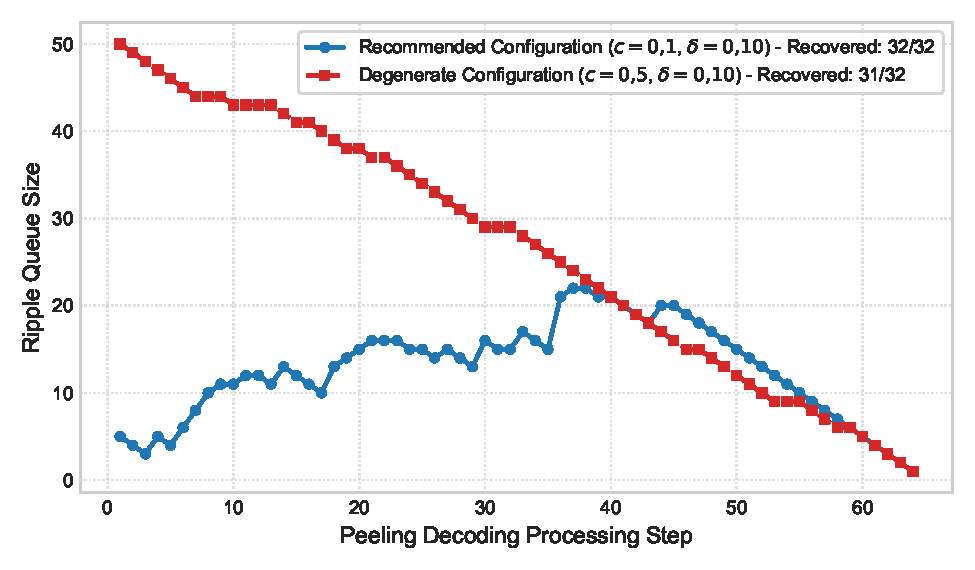
\includegraphics[width=0.78\textwidth]{figuras/grafico_ripple.pdf}
    \caption{Evolution of ripple queue length across peeling decoding steps ($K = 32$, $\epsilon = 1.00$, $p_{\text{loss}} = 0.0$). Single illustrative run; aggregate success rate for $c = 0.5$ is 0\% (0/100).}
    \label{fig:dinamica_ripple}
    \fonte{Prepared by the author (2026).}
\end{figure}

Analysis of Figure~\ref{fig:dinamica_ripple} and Table~\ref{tab:ripple_metricas} clarifies operational differences between aggregate means and individual runs:
\begin{enumerate}
    \item The ``Queue Peak ($Q_{\max}$)'' metric in Table~\ref{tab:ripple_metricas} reports the sample mean of maximum queue lengths reached across 100 independent runs under intermediate overhead $\epsilon = 0.50$. In contrast, Figure~\ref{fig:dinamica_ripple} displays the trajectory of a single execution under full overhead ($\epsilon = 1.00$), explaining why individual curve peaks differ from tabulated $\epsilon = 0.50$ means;
    \item Under recommended settings ($c = 0.1$, $\epsilon = 1.00$), the queue is replenished steadily throughout decoding, reaching a moderate peak of 22 elements and sustaining continuous releases until all 32 blocks are recovered (32/32);
    \item Under $c = 0.5$, the RSD mode collapses to $m = \lfloor 32/16.32 \rfloor = 1$, where approximately 73\% of droplets are generated with degree 1. This floods the initial queue (peak of 50 elements). Decoding executes for 64 iterations dequeuing packets, but most represent redundant droplets covering previously resolved blocks. Due to the scarcity of intermediate-degree droplets needed to interlink remaining blocks via XOR, decoding halted with one unresolved block (31 of 32 recovered) once unit equations were exhausted;
    \item The minimum queue size ($Q_{\min}$) being recorded as 1.0 across all rows in Table~\ref{tab:ripple_metricas} is an artifact of instrumentation: sampling occurs inside the decoding loop (\texttt{while ripple:}), when the queue inherently holds at least one active element. Final emptying (size zero) represents the loop termination condition.
\end{enumerate}

\section{Overhead versus Success Rate}
\label{sec:results_overhead_success_rate}

The relationship between transmitted relative overhead $\epsilon = (N - K)/K$ and decoding success probability is a defining characteristic of fountain codes. Across the experimental grid, $N$ denotes the count of screened, transmitted oligonucleotides ($N = N_{\text{tx}}$). LT code theory proves that required relative overhead diminishes asymptotically with $K$. In finite block regimes, the empirical relationship must be characterized experimentally across evaluated overhead levels ($\epsilon \in \{0.25, 0.50, 1.00\}$), manifesting as a gradual transition.

Table~\ref{tab:overhead_sucesso} summarizes success rates obtained for different overhead tiers over an ideal channel ($p_{\text{loss}} = 0.0$) with $\delta = 0.10$.

\begin{table}[htbp]
    \centering
    \small
    \caption{Decoding success rate as a function of sent overhead ($\delta = 0.10$, $p_{\text{loss}} = 0.0$).}
    \label{tab:overhead_sucesso}
    \begin{tabular}{ccccc}
        \toprule
        \multirow{2}{*}{\textbf{$K$}} & \multirow{2}{*}{\textbf{$c$}} & \multicolumn{3}{c}{\textbf{Success Rate (\%) by Overhead Level}} \\
        \cmidrule(lr){3-5}
        & & \textbf{$\epsilon = 0.25$} & \textbf{$\epsilon = 0.50$} & \textbf{$\epsilon = 1.00$} \\
        \midrule
        16 & 0.1 & 8.0 & 49.0 & 90.0 \\
        16 & 0.3 & 36.0 & 64.0 & 91.0 \\
        16 & 0.5 & 0.0 & 4.0 & 24.0 \\
        16 & 0.8 & 0.0 & 0.0 & 7.0 \\
        \midrule
        32 & 0.1 & 30.0 & 85.0 & 100.0 \\
        32 & 0.3 & 38.0 & 68.0 & 93.0 \\
        32 & 0.5 & 0.0 & 0.0 & 0.0 \\
        32 & 0.8 & 0.0 & 0.0 & 4.0 \\
        \midrule
        64 & 0.1 & 19.0 & 88.0 & 100.0 \\
        64 & 0.3 & 10.0 & 57.0 & 97.0 \\
        64 & 0.5 & 0.0 & 27.0 & 82.0 \\
        64 & 0.8 & 0.0 & 0.0 & 3.0 \\
        \bottomrule
    \end{tabular}
    \fonte{Prepared by the author (2026).}
\end{table}

Figure~\ref{fig:overhead_sucesso} illustrates sample points and guide curves of success rate as a function of transmitted overhead across source block counts ($K = 16$, $K = 32$, and $K = 64$) and constants $c \in \{0.1, 0.3, 0.5, 0.8\}$.

\begin{figure}[htbp]
    \centering
    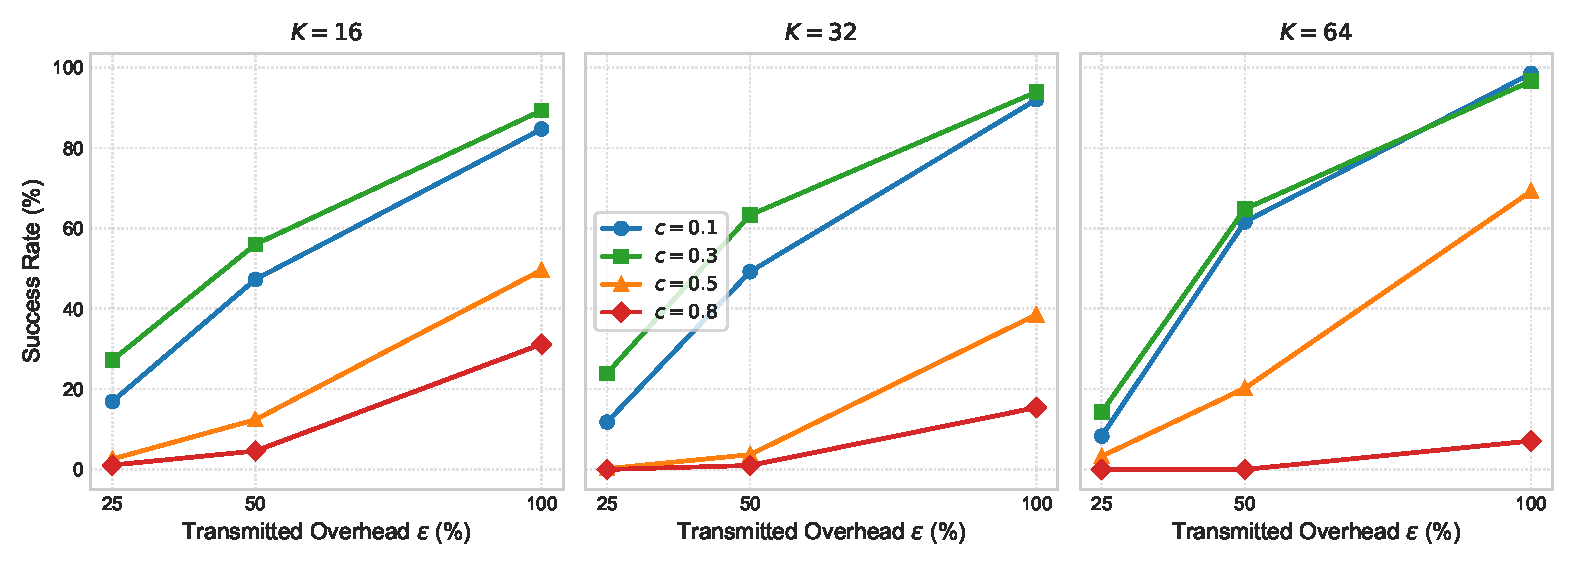
\includegraphics[width=\textwidth]{figuras/grafico_overhead_sucesso.pdf}
    \caption{Decoding success rate as a function of sent overhead ($\delta = 0.10$, $p_{\text{loss}} = 0.0$).}
    \label{fig:overhead_sucesso}
    \fonte{Prepared by the author (2026).}
\end{figure}

The visualization in Figure~\ref{fig:overhead_sucesso} demonstrates that, across evaluated overhead levels ($\epsilon \in \{0.25, 0.50, 1.00\}$), response curves steepen noticeably as $K$ increases:
\begin{itemize}
    \item For $K = 16$, the transition is gradual, peaking at 91\% even under $\epsilon = 1.00$, illustrating heightened vulnerability to stochastic variance in small block counts;
    \item For $K = 32$ and $K = 64$, the $c = 0.1$ curve climbs rapidly from $\epsilon = 0.25$, reaching 85\%--88\% at $\epsilon = 0.50$ and consolidating at 100\% under $\epsilon = 1.00$ (95\% CI: $[96.4\%, 100.0\%]$);
    \item Curves for $c = 0.8$ remain pinned near the horizontal axis (near-zero success) across virtually all overhead levels.
\end{itemize}

\subsection{Structural Performance Discrepancy with $c = 0.5$ between $K = 32$ and $K = 64$}

One of the most revealing behaviors documented in Table~\ref{tab:overhead_sucesso} occurs with $c = 0.5$ under overhead $\epsilon = 1.00$: while for $K = 32$ the recovery rate is zero ($0.0\%$, 95\% CI: $[0.0\%, 3.6\%]$), for $K = 64$ the system achieves $82.0\%$ success (95\% CI: $[73.1\%, 89.0\%]$).

This contrast stems directly from how mode index $m = \lfloor K/R \rfloor$ scales with $K$:
\begin{itemize}
    \item For $K = 32$, we have $R = 0.5 \ln(32/0.10)\sqrt{32} \approx 16.32$, yielding $m = \lfloor 32 / 16.32 \rfloor = 1$. The entire corrective term $\tau(d)$ collapses onto degree 1. The RSD generates approximately 73\% unit-degree droplets, severely depleting degree-2 and higher combinatoric droplets needed to interlink remaining blocks. Lacking sufficient graph connectivity, 0 successes were observed in 100 trials ($0.0\%$, 95\% CI: $[0.0\%, 3.6\%]$);
    \item For $K = 64$, we obtain $R \approx 25.85$, yielding $m = \lfloor 64 / 25.85 \rfloor = 2$. Corrective values evaluate to $\tau(1) \approx 0.404$ and $\tau(2) \approx 2.243$, with $\tau(d) = 0$ for all $d > 2$. Normalizing $\rho(d) + \tau(d)$ produces $\mu(1) \approx 0.115$ and $\mu(2) \approx 0.752$, with mean degree $\bar{d} \approx 2.64$. This distribution avoids collapsing onto degree 1: because three-quarters of the probability mass concentrates on degree-2 droplets, they act as primary catalytic drivers for peeling (reducing to degree 1 once one neighbor is resolved), sustaining peeling progress and achieving $82.0\%$ success under $\epsilon = 1.00$.
\end{itemize}

This observation supports the hypothesis that block scale $K$ can qualitatively alter the viability of a given RSD parameterization, demonstrating that parameter choices unsuited for small messages may become partially viable as graph dimensions expand.

\section{Impact of Parameters $c$ and $\delta$}
\label{sec:results_impact_c_delta}

Parameters $c$ and $\delta$ govern the Robust Soliton Distribution through corrective component $\tau(d)$ and scale parameter $R = c \ln(K/\delta)\sqrt{K}$. Parameter $c$ scales $R$, while $\delta$ sets an asymptotic upper bound on decoding failure probability.

Table~\ref{tab:impacto_c_delta} details the systematic impact of $c$ and $\delta$ on system metrics for $K = 32$, under fixed overhead $\epsilon = 0.50$ and lossless channel ($p_{\text{loss}} = 0.0$).

\begin{table}[htbp]
    \centering
    \small
    \caption{Impact of $c$ and $\delta$ on decoding metrics ($K = 32$, $\epsilon = 0.50$, $p_{\text{loss}} = 0.0$).}
    \label{tab:impacto_c_delta}
    \resizebox{\textwidth}{!}{%
    \begin{tabular}{ccccccc}
        \toprule
        \textbf{$c$} & \textbf{$\delta$} & \textbf{$R$} & \shortstack{\textbf{Theoretical Mean Degree}\\\textbf{($\mathbb{E}_\mu[D]$)}} & \textbf{Mean XORs} & \textbf{Peak Ripple} & \textbf{Success (\%)} \\
        \midrule
        0.1 & 0.10 & 3.263 & 4.945 & 196.0 & 10.5 & 85.0 \\
        0.1 & 0.01 & 4.566 & 4.961 & 129.8 & 7.2 & 33.0 \\
        0.3 & 0.10 & 9.789 & 3.103 & 140.2 & 14.3 & 68.0 \\
        0.3 & 0.01 & 13.697 & 2.361 & 106.4 & 17.2 & 41.0 \\
        0.5 & 0.10 & 16.315 & 1.850 & 75.7 & 38.2 & 0.0 \\
        0.5 & 0.01 & 22.828 & 1.469 & 60.6 & 40.9 & 0.0 \\
        0.8 & 0.10 & 26.104 & 1.552 & 65.4 & 39.9 & 0.0 \\
        0.8 & 0.01 & 36.525 & 1.295 & 56.2 & 42.4 & 0.0 \\
        \bottomrule
    \end{tabular}%
    }
    \fonte{Prepared by the author (2026).}
\end{table}

Figure~\ref{fig:impacto_c_delta} illustrates the joint behavior of theoretical mean degree ($\mathbb{E}_\mu[D]$) and decoding success rate as functions of $c$, for both evaluated $\delta$ levels ($0.10$ and $0.01$).

\begin{figure}[htbp]
    \centering
    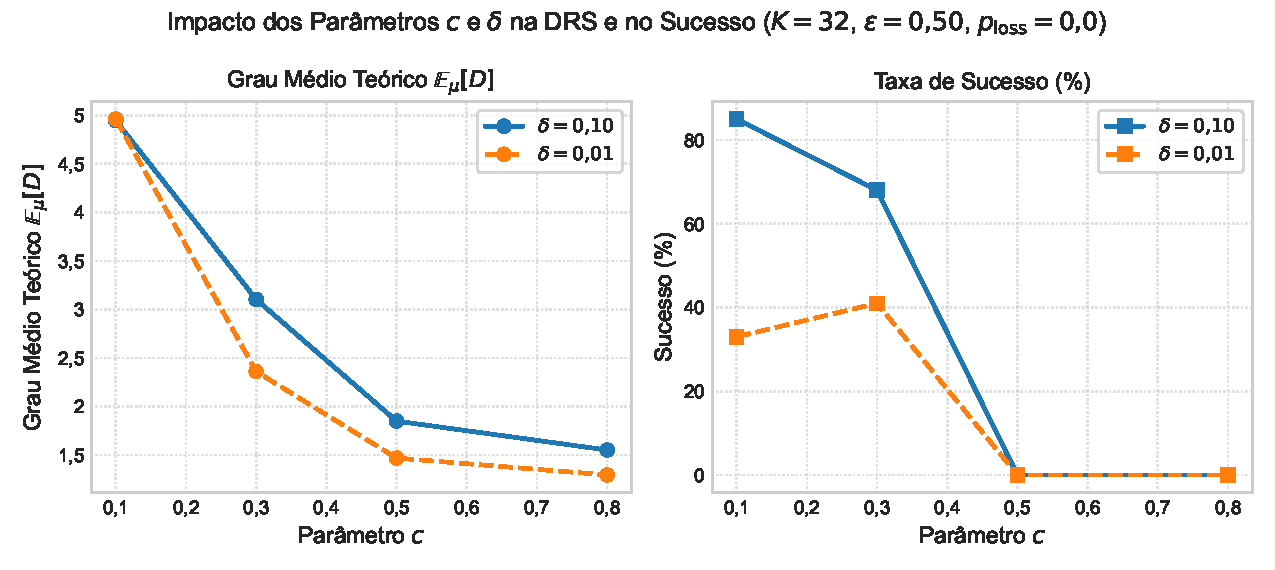
\includegraphics[width=0.88\textwidth]{figuras/grafico_impacto_c_delta.pdf}
    \caption{Impact of parameters $c$ and $\delta$ on degree distribution and success rate ($K = 32$, $\epsilon = 0.50$, $p_{\text{loss}} = 0.0$).}
    \label{fig:impacto_c_delta}
    \fonte{Prepared by the author (2026).}
\end{figure}

The relationship in Figure~\ref{fig:impacto_c_delta} highlights the mechanics of the RSD in finite block regimes:
\begin{enumerate}
    \item \textbf{Distribution Degeneracy for $c \ge 0.5$}: When $c$ takes elevated values ($0.5$ or $0.8$), $R$ reaches $16.32$ or $26.10$ for $K = 32$. Because $R$ approaches or exceeds half of $K$, corrective mode $m = \lfloor K/R \rfloor$ collapses to $1$. For $c = 0.5$, approximately 73.1\% of normalized mass concentrates on degree 1 ($\mu(1) \approx 0.731$, $\mu(2) \approx 0.139$); for $c = 0.8$, degree-1 concentration worsens to $\mu(1) \approx 0.825$ ($\mu(2) \approx 0.090$). Consequently, theoretical mean degree $\mathbb{E}_\mu[D]$ plummets from $4.95$ to $1.85$ and $1.55$ (closely mirrored by sampled mean degree $\bar{d}_{\text{emp}}$). With insufficient combinatoric connectivity to sustain peeling, 0 successes were observed in 100 runs under $K=32, \epsilon=0.50, p_{\text{loss}}=0.0$ (95\% CI: $[0.0\%, 3.6\%]$);
    
    \item \textbf{Effect of $\delta$ and Low-Degree Dynamics}: Contrary to the intuition that smaller $\delta$ would concentrate mass on low degrees, reducing $\delta$ from $0.10$ to $0.01$ under $c = 0.1$ leaves theoretical mean degree virtually unchanged ($\mathbb{E}_\mu[D]$ shifts from $4.945$ to $4.961$). The sharp performance drop (success falling from $85.0\%$ to $33.0\%$) is consistent with probability mass redistribution, including reduced degree-2 probability ($\mu(2)$ decreases from $\approx 0.338$ to $\approx 0.257$) and mode shift ($m$ retreats from $9$ to $7$ as $R$ expands from $3.26$ to $4.57$). With fewer degree-2 droplets to replenish the queue following initial releases, peak ripple drops ($7.2$ vs. $10.5$), exhausting prematurely;
    
    \item \textbf{Relationship with XOR Operations}: As mean degree falls, average XOR operations executed during decoding also decrease (from 196.0 to 65.4). However, this computational savings reflects premature decoder stall due to connection exhaustion rather than algorithmic efficiency.
\end{enumerate}

Characterizing $c = 0.1$ and $\delta = 0.10$ as the most effective configuration must be contextualized within the evaluated parameter domain. While this combination proved clearly superior for $K = 32$ and $K = 64$ under intermediate overheads ($\epsilon = 0.50$ and $\epsilon = 1.00$), it does not represent an unconstrained global optimum. First, $c = 0.1$ was the lowest value tested, leaving $c < 0.1$ unexamined. Second, in the specific case of $K = 16$ under constrained overhead ($\epsilon = 0.25$) over an ideal channel, $c = 0.3$ statistically outperformed $c = 0.1$, recording $36.0\%$ success versus $8.0\%$ (two-tailed Fisher's exact test, $p = 2.2 \times 10^{-6}$); for $K = 32$, the observed difference between $c = 0.3$ and $c = 0.1$ ($38.0\%$ vs. $30.0\%$) was not statistically significant ($p \approx 0.30$, two-tailed Fisher's test). For $K = 16$, the advantage of $c = 0.3$ under constrained redundancy stems from RSD dynamics: under $c = 0.1$, $R \approx 2.03$ and mode index sits at $m = 7$, yielding $\mu(1) \approx 0.112$ and $\mu(2) \approx 0.333$; switching to $c = 0.3$, $R \approx 6.09$ and the mode index shifts to $m = 2$, slightly increasing $\mu(1)$ to $0.150$ and concentrating a substantial $\mu(2) \approx 0.701$ of probability mass on degree-2 droplets (more than double $0.333$). This high degree-2 concentration provides a rich reserve of binary equations ready to become degree-1 as soon as the first source block is resolved, sustaining continuous peeling momentum and preventing early stall under tight packet budgets.

\section{System Resilience to Channel Losses}
\label{sec:results_system_resilience}

The ability to operate over lossy channels without retransmission feedback is a primary motivation for fountain code architectures. To quantify this tolerance, the simulator was evaluated under stochastic erasure probabilities $p_{\text{loss}} \in \{0.0, 0.10, 0.20\}$, representing erasure rates up to 20\% per transmitted oligonucleotide.

Table~\ref{tab:resiliencia_canal} compares success rates and XOR operations under channel losses for the reference parameterization ($c = 0.1$, $\delta = 0.10$) across overhead levels.

\begin{table}[htbp]
    \centering
    \small
    \caption{System resilience under stochastic channel losses ($c = 0.1$, $\delta = 0.10$).}
    \label{tab:resiliencia_canal}
    \begin{tabular}{cccccc}
        \toprule
        \textbf{$K$} & \textbf{Overhead ($\epsilon$)} & \textbf{$p_{\text{loss}} = 0.0$} & \textbf{$p_{\text{loss}} = 0.10$} & \textbf{$p_{\text{loss}} = 0.20$} & \textbf{XORs ($p_{\text{loss}} = 0.20$)} \\
        \midrule
        16 & 0.25 & 8.0\% & 5.0\% & 0.0\% & 8.6 \\
        16 & 0.50 & 49.0\% & 32.0\% & 15.0\% & 22.4 \\
        16 & 1.00 & 90.0\% & 83.0\% & 70.0\% & 72.2 \\
        \midrule
        32 & 0.25 & 30.0\% & 10.0\% & 2.0\% & 51.2 \\
        32 & 0.50 & 85.0\% & 55.0\% & 27.0\% & 107.9 \\
        32 & 1.00 & 100.0\% & 99.0\% & 89.0\% & 207.0 \\
        \midrule
        64 & 0.25 & 19.0\% & 1.0\% & 0.0\% & 60.5 \\
        64 & 0.50 & 88.0\% & 52.0\% & 16.0\% & 172.7 \\
        64 & 1.00 & 100.0\% & 98.0\% & 92.0\% & 520.1 \\
        \bottomrule
    \end{tabular}
    \fonte{Prepared by the author (2026).}
\end{table}

Figure~\ref{fig:resiliencia_canal} illustrates recovery rate as a function of $p_{\text{loss}}$ across the three overhead tiers ($\epsilon = 0.25$, $\epsilon = 0.50$, and $\epsilon = 1.00$) for $K = 32$ and $K = 64$.

\begin{figure}[htbp]
    \centering
    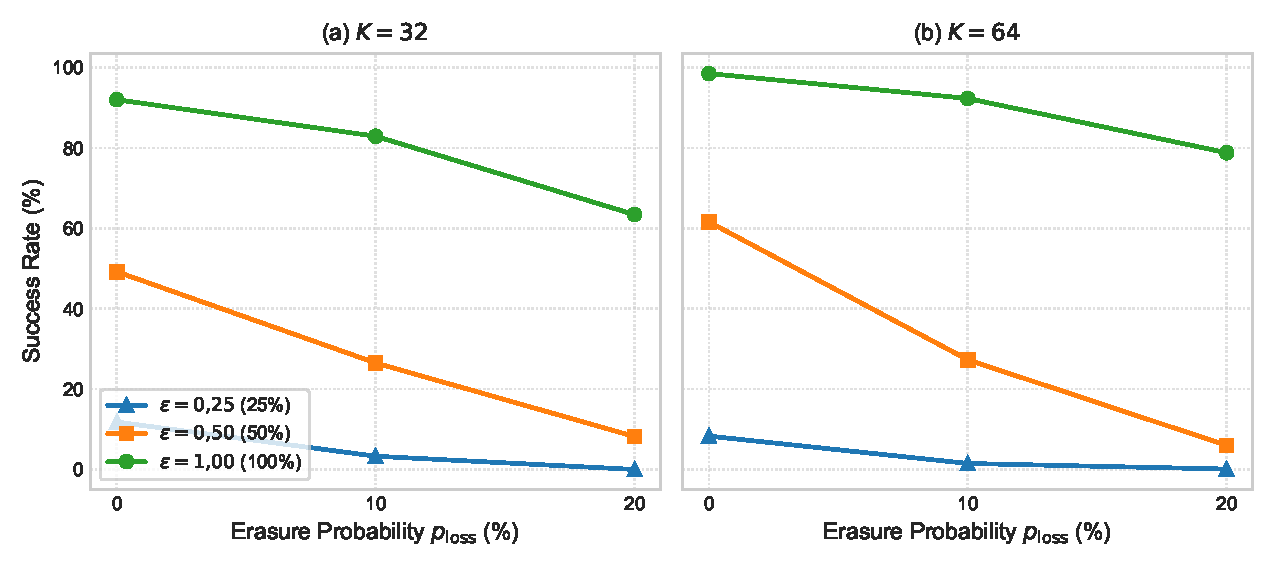
\includegraphics[width=0.88\textwidth]{figuras/grafico_resiliencia.pdf}
    \caption{System resilience under stochastic channel losses ($c = 0.1$, $\delta = 0.10$).}
    \label{fig:resiliencia_canal}
    \fonte{Prepared by the author (2026).}
\end{figure}

The results show that a packet erasure channel with loss probability $p_{\text{loss}}$ directly reduces effective received overhead. Mathematically, the expected number of arriving droplets is $\mathbb{E}[N_{\text{rx}}] = N_{\text{tx}}(1 - p_{\text{loss}})$, yielding an expected effective overhead $\mathbb{E}[\epsilon_{\text{rx}}] = (1 + \epsilon_{\text{tx}})(1 - p_{\text{loss}}) - 1$.

When transmitting with nominal overhead $\epsilon = 1.00$ ($N_{\text{tx}} = 2K$), even under erasure probability $p_{\text{loss}} = 0.10$, the decoder still receives on average $1.8K$ droplets ($\mathbb{E}[\epsilon_{\text{rx}}] = 0.80$). Because this volume remains well above the threshold required to sustain peeling across evaluated configurations, success rates remain virtually unaffected: 99\% for $K = 32$ and 98\% for $K = 64$. Even under $p_{\text{loss}} = 0.20$, the system sustains 89\% recovery for $K = 32$ and 92\% for $K = 64$.

Conversely, configurations operating with intermediate nominal overhead ($\epsilon = 0.50$, marginal for full recovery) degrade sharply under losses: for $K = 64$, under $p_{\text{loss}} = 0.10$ success drops from 88\% to 52\%, and under $p_{\text{loss}} = 0.20$ plummets to 16\%. This behavior reinforces a core design principle: in physical DNA storage channels subject to molecular decay and sequencing dropout, overhead margins must be provisioned according to anticipated sequencing losses.

\section{Computational Cost}
\label{sec:results_computational_cost}

Computational cost was quantified through two complementary metrics: total decoder execution runtime (in milliseconds) and XOR operation counts executed across data blocks.

Measured execution time covers complete execution of \texttt{decoder.decodificar()}, comprising: (1) nucleotide-to-byte conversion; (2) obfuscated seed parsing; (3) CRC-8 verification; (4) neighbor index regeneration; (5) inverted adjacency index construction; and (6) peeling iterations with XOR propagation.

Table~\ref{tab:custo_computacional} consolidates total decoding runtime and XOR effort observed across 100 repetitions with $c = 0.1$, $\delta = 0.10$, overhead $\epsilon = 1.00$, and ideal channel ($p_{\text{loss}} = 0.0$). Reported runtime and XOR means include all 100 runs per configuration in the version under commit \texttt{bb2f0ab}, regardless of outcome (success or failure). Each counted XOR operation represents peeling propagation effort, corresponding to exact calls to \texttt{xor\_blocos} across $L = 4$-byte blocks during edge removal (\texttt{outro["indices"].remove(idx\_bloco)}). Logic operations for CRC-8 verification and descrambling occur during framing parsing and are excluded from this counter. Because averages include all runs, lower mean cost can occasionally reflect premature stall in unrecovered instances rather than intrinsic efficiency. Individual timing and operation records are archived in \texttt{tempos\_brutos\_decodificacao.json}, from which sample mean, sample standard deviation, median, and extreme values were computed via \texttt{salvar\_estatisticas\_custo.py}.

\begin{table}[htbp]
    \centering
    \footnotesize
    \caption{Total decoder computational cost by block count ($c = 0.1$, $\delta = 0.10$, $\epsilon = 1.00$, $p_{\text{loss}} = 0.0$).}
    \label{tab:custo_computacional}
    \resizebox{\textwidth}{!}{%
    \begin{tabular}{ccccccc}
        \toprule
        \textbf{$K$} & \textbf{Mean Runtime (ms)} & \textbf{Std. Dev. (ms)} & \textbf{Median (ms)} & \textbf{Min--Max (ms)} & \textbf{Mean XORs} & \textbf{XORs/Block} \\
        \midrule
        16 & 0.84 & 0.04 & 0.84 & 0.71 -- 0.99 & 107.6 & 6.73 \\
        32 & 1.79 & 0.12 & 1.77 & 1.65 -- 2.48 & 270.8 & 8.46 \\
        64 & 3.60 & 0.19 & 3.55 & 3.35 -- 4.51 & 688.4 & 10.76 \\
        \bottomrule
    \end{tabular}%
    }
    \fonte{Prepared by the author (2026).}
\end{table}

Figure~\ref{fig:custo_computacional} illustrates average decoding runtime (with $\pm 1$ standard deviation error bars) and XOR operations as functions of block count $K$.

\begin{figure}[htbp]
    \centering
    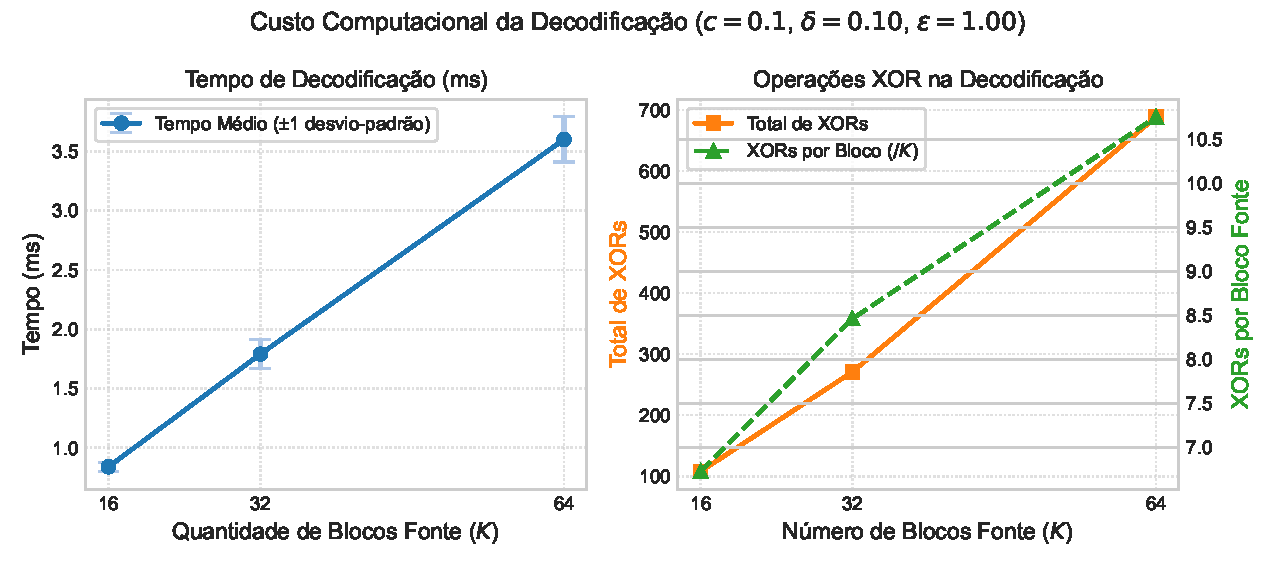
\includegraphics[width=0.88\textwidth]{figuras/grafico_custo_computacional.pdf}
    \caption{Total decoder computational cost as a function of $K$ ($c = 0.1$, $\delta = 0.10$, $\epsilon = 1.00$, $p_{\text{loss}} = 0.0$).}
    \label{fig:custo_computacional}
    \fonte{Prepared by the author (2026).}
\end{figure}

LT code theory establishes asymptotic decoding complexity of order $O(K \ln(K/\delta))$ symbol operations~\cite{luby2002}. Empirical data gathered across the narrow range $K \le 64$ align with this theoretical trend, though a three-point sample does not conclusively substantiate asymptotic scaling:
\begin{itemize}
    \item Mean decoding runtime remained within milliseconds (from 0.84~ms for $K = 16$ to 3.60~ms for $K = 64$), staying well below 5~ms across benchmark runs on the host system (Windows~11, interpreted Python 3.12);
    \item Average XOR operations per source block grew moderately ($6.73 \to 8.46 \to 10.76$), characterizing computational work under the inverted bipartite graph indexing;
    \item Low runtime dispersion (standard deviations between 0.04 and 0.19~ms) and close agreement between mean and median indicate stable executions, with variations reflecting OS thread scheduling and interpreter execution behavior.
\end{itemize}

These results characterize short study instances ($K \le 64$), tailored for controlled, pedagogical experimentation. They cannot be directly extrapolated to large-scale files (scaling $K \times L$ to megabytes or gigabytes), where memory allocation and Python interpreter overhead warrant compiled implementations in C/C++, Rust, or dedicated FPGA hardware acceleration.

\section{Limitations of the Results}
\label{sec:results_limitations}

To uphold academic rigor, the scope and limitations of the presented findings must be explicitly delimited:

\begin{enumerate}
    \item \textbf{Simplified Communication Channel}: The simulator models DNA storage as an abstract memoryless Binary Erasure Channel (BEC), where droplets arrive intact or are entirely erased. In physical wet-lab practice, synthesis, storage, and sequencing suffer from substitution errors, insertions, deletions (indels), and non-uniform sequence-dependent coverage bias~\cite{heckel2019, shomorony2022}. Resilience results reported herein reflect performance under idealized packet erasures without phase noise or point mutations. Moreover, evaluated erasure probabilities represent controlled simulation scenarios rather than calibrated estimates for a specific laboratory protocol;
    
    \item \textbf{Source Block Scale ($K$)}: Experimental batteries focused on $K \in \{16, 32, 64\}$. This choice enabled exhaustive exploration of a 216-combination factorial matrix with 100 repetitions per point (21,600 trials). While suitable for analyzing transition dynamics and RSD behavior in small regimes, real-world DNA archiving platforms~\cite{erlich2017} operate with $K$ on the order of tens or hundreds of thousands of blocks, where boundary effects diminish and required overhead drops to 5\%--10\%;
    
    \item \textbf{High-Level Language Implementation}: The simulator was developed in pure Python 3 for modularity, didactic clarity, maintainability, and reproducibility. Consequently, runtime measurements reflect CPython interpretation overhead rather than the performance obtainable via optimized C/C++, Rust, or FPGA implementations;
    
    \item \textbf{Seed Search Space and Net Storage Density}: A 16-bit seed header limits addressing capacity to $2^{16} = 65,536$ unique seed values. Under biological screening (rejecting $\approx 40.2\%$ of candidates), the usable oligonucleotide universe is approximately 39,000 sequences. Furthermore, the prototype's framing structure (2 bytes seed, $L=4$ bytes payload, 1 byte CRC-8, totaling 7 bytes or 28 nucleotides) yields a payload density of $\approx 1.14$ bits per nucleotide ($32\text{ bits} / 28\text{ nt}$) per transmitted strand prior to accounting for LT redundancy ($1+\epsilon$), screening rejections, or PCR primers, illustrating the relative weight of headers in short oligonucleotides;
    
    \item \textbf{Stochastic Portability across Runtimes}: Reliance on Python's standard \texttt{random} module ensures strict reproducibility when runtime version is held fixed (Python~3.12). However, CPython specifications guarantee long-term repeatability only for the core floating-point generator \texttt{random()}, while sampling routines may undergo subtle implementation refinements across minor versions. For decadal digital preservation or FPGA migration, an autonomous PRNG specification (such as an arithmetic LFSR or PCG/xoshiro generator) is recommended;
    
    \item \textbf{Evaluation of Screened Pipeline}: The biological screening module remained uniformly active across all configurations in the main factorial grid, reflecting physical synthesis constraints. The study evaluated the screened pipeline and characterized accepted candidate distributions in a dedicated trial, without isolating the direct causal performance delta between transmission with screening versus an unconstrained transmission without screening.
\end{enumerate}
